\chapter{BCI-Framework}\label{ch:chapter_4}

In computer programming, a framework is an abstraction in which software, providing generic functionality, can be selectively changed by additional user-written code, thus providing application-specific software. It supply a standard way to build and deploy applications and is a universal, reusable software environment that allow particular functionality as part of a larger software platform to facilitate the development of software applications, products and solutions. Frameworks-based software may include support programs, compilers, code libraries, toolsets, and application programming interfaces (\gls*{API}s) that bring together all the different components to carry up the development of a project or system \cite{soni2017full} without the need to looks out of the framework.

This chapter describe the implementation of a independent \gls*{BCI} software that consists of a distributed processing tool, stimuli delivery, psychophysiological experiments designer and real-time data visualizations for \textit{OpenBCI}. 

We purpose an open-source tool for the acquisition of EEG/EMG/ECG signals and designed to work with \textit{OpenBCI’s Cyton} board, the main core of this software lies on \footcite{OpenBCI-Stream}{https://openbci-stream.readthedocs.io} and a library designed to handle all the low-level hardware features to extend the hardware capabilities with high-level programming libraries developed in \hyperref[ch:chapter_2]{Chapter 2}. \textit{BCI-Framework} comprises a \gls*{GUI} with a set of individual computational processes (distributed or in a single machine), that feeds visualizations, serve stimuli delivery, handle acquisitions, storage data and/or process data in real-time. Additionally has a built-in development environment and a set of libraries that the user can implement to create their specific functionalities.

\textit{BCI-Framework} as well as all \gls*{BCI} applications implies the participation of at least two kind of users that will be widely used in this chapter: 
(i) the \textit{user} role refers to the person that manipulate the framework to execute experiments;
(ii) the \textit{patient} is the subject from whom the EEG data is being acquired;
(iii) a third profile can be assigned to a \textit{developer} or \textit{researcher}, this subject use the framework extensibilities to create new experiments and visualizations.


%======================================================================
\section{Software description}

BCI-Framework is a desktop application that was developed entirely using \textit{Python} and the \gls*{GUI} was implemented initially on PySide2 and updated to run under the latest stable release of \footcite{PySide6}{https://wiki.qt.io/Qt\_for\_Python}. In fact all libraries implemented are free (as in freedom) or at least \textit{Open-Source}. The software architecture is modular and designed taking into account the scalability and the configurability. Almost all components run on independent computational process and are connected to the main interface through websockets or simple \textit{HTTP} petitions.

The major feature of \textit{BCI-Framework} is the capability to implement a complete EEG-based BCI system in a single software application. This achievement, in part, is due the dedicated support to \textit{OpenBCI Cyton} board and the \hyperref[chap3:isolated-acquisition]{Isolated acquisition} that was described and implemented in Chapter 3. This feature leaves to the main machine, the one that run the framework interface, to keep all the resources to perform visualisations, processings and run a stimuli delivery server. And at the same time have a reliable flow of data.

\textit{BCI-Framework} use a set of background services that run independent of each other, some process are initialised from inside the framework and others from outside, all process run under a distributed network. All this backend services exchange information using \textit{Kafka} or \textit{Websockets}, it depends on the priority level or the amount of the information transmitted. 

% The two main backends developed with the intention to be integrated and implemented in the development of \textit{BCI-Framework} are the related with the real-time visualizations and the stimuli delivery.


%----------------------------------------------------------------------
\subsection{Real-time visualizations backend}\label{ch4:realtime_visualizations_backend}

This feature uses the \footcite{Matplotlib}{https://matplotlib.org/} backend through \footcite{FigureStream}{https://figurestream.readthedocs.io/}  a python module developed explicitly for this framework, that serve the visualization using a simple HTTP real-time streaming. This module creates a static endpoint and the image is updated like in a video streaming, this is a synchronous process, this means that the user has the control and the responsibility to feed the streaming frame by frame.

In background, a \footcite{Flask}{https://flask.palletsprojects.com/} application is running and serving the endpoint with the streaming plot for all users in the network, then, the visualizations can be both, consumed and generated from any terminal. This feature is ideal for distributed systems, since, costly real-time visualizations can be executed on a independent hardware.

The development of this backend module is described in the appendix \hyperref[appendix:matplotlib-figurestream]{Matplotlib-FigureStream}.




%----------------------------------------------------------------------
\subsection{Stimuli delivery backend}\label{ch4:stimuli_delivery_backend}

This environment is based on \textit{HTML} and \textit{JavaScript}, is basically a dynamic web application. However, in order to standardize all user scripts into a single language, this feature use \footcite{Brython}{https://brython.info/index.html}, a \textit{Python3} implementation for client-side web programming. This tool able to the user to write web applications, however, is necessary a server running with the dependencies and the library itself. With the intention to simplify the implementation and the start up of \textit{Brython} projects, a Python module called \hyperref[appendix:brython-radiant]{Brython-Radiant framework} was implemented that solve this isssues. This module is a \textit{Brython} framework for the quick development of web apps with pure \textit{Python/Brython} syntax so there is no need to care about \textit{HTML}, \textit{CSS}, or \textit{JavaScript}. Runs over \footcite{Tornado}{https://www.tornadoweb.org} and include support to \textit{Websockets}, \textit{Local Python Scripts} and \footcite{Material Design Components}{https://material.io/develop/web}. This is basically a set of scripts that allows the same script run from \textit{Python} and \textit{Brython}, when its running under \textit{Python} a \textit{Tornado} server is created and configure the local path for serving static files, and a custom \textit{HTML} template is configured in runtime to import the same script, this time, interpreted by \textit{Brython}.

\textit{Brython-Radiant} able to the user to create with pure Python and a single script a complete web application that can interact with the native Python environment. And when run under a network-based implementation allows to be consumed from any terminal. 


%======================================================================
\subsection{Development environment}

The main interface is divided into two high-level functionalities: 
(i) Real-time analysis, to collect and process data, include and interface to handle custom visualizations and serve \textit{Kafka} generators;
% (ii) Timelock analysis, to process data off-line and generate reports;
(ii) Stimuli delivery, to serve remote audiovisual stimuli and configure experiments.
This functionalities includes a set of visualizations and basic paradigms by default, instead of being rigidly included in the interface, they are in fact fully editable and configurable, even new ones can be created from scratch as an extension. All scripts are accessible under an integrated development environment.

\begin{figure}
\begin{centering}
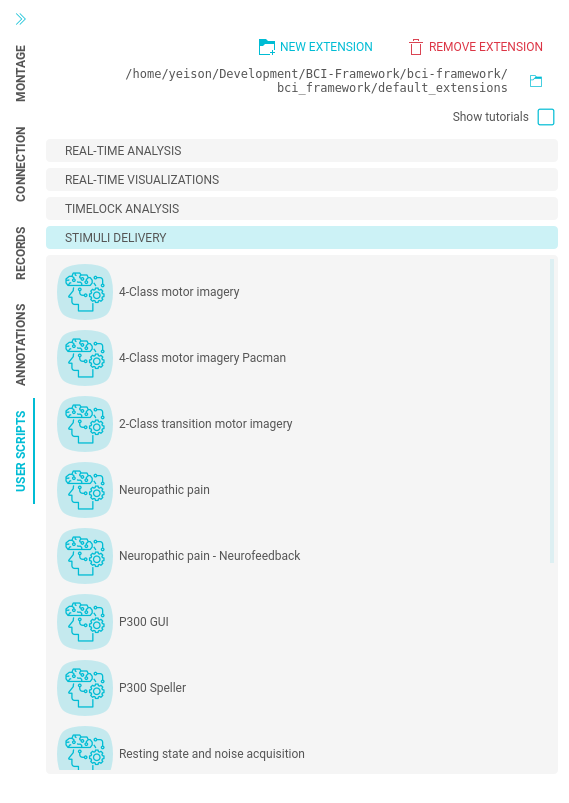
\includegraphics[width=0.5\textwidth]{Cap4/Figures/development_environment_extensions.png}
\par\end{centering}
\caption[BCI-Framework: Extensions panel]{BCI-Framework: The extensions panel is used to access to all visualizations and stimuli delivery paradigms source code, as well to create a new ones from scratch. }
\label{fig:development_environment_extension}
\end{figure}

The development environment is one of the most outstanding features of \textit{BCI-Framework}, this environment able to developers to implement custom data analysis, real-time visualizations and, design custom stimuli delivery experiments or paradigms without leaving the main interface. This is achieved by the development and the implementation of an \gls*{API} that interact with the framework parameters, the real-time data stream and with the users. Figure \ref{fig:development_environment} shows a capture of the integrated development environment, that consist of a full Python syntax highlighting, a previsualization area, a directory tree navigator, and a debugging console.




\begin{figure}
\begin{centering}
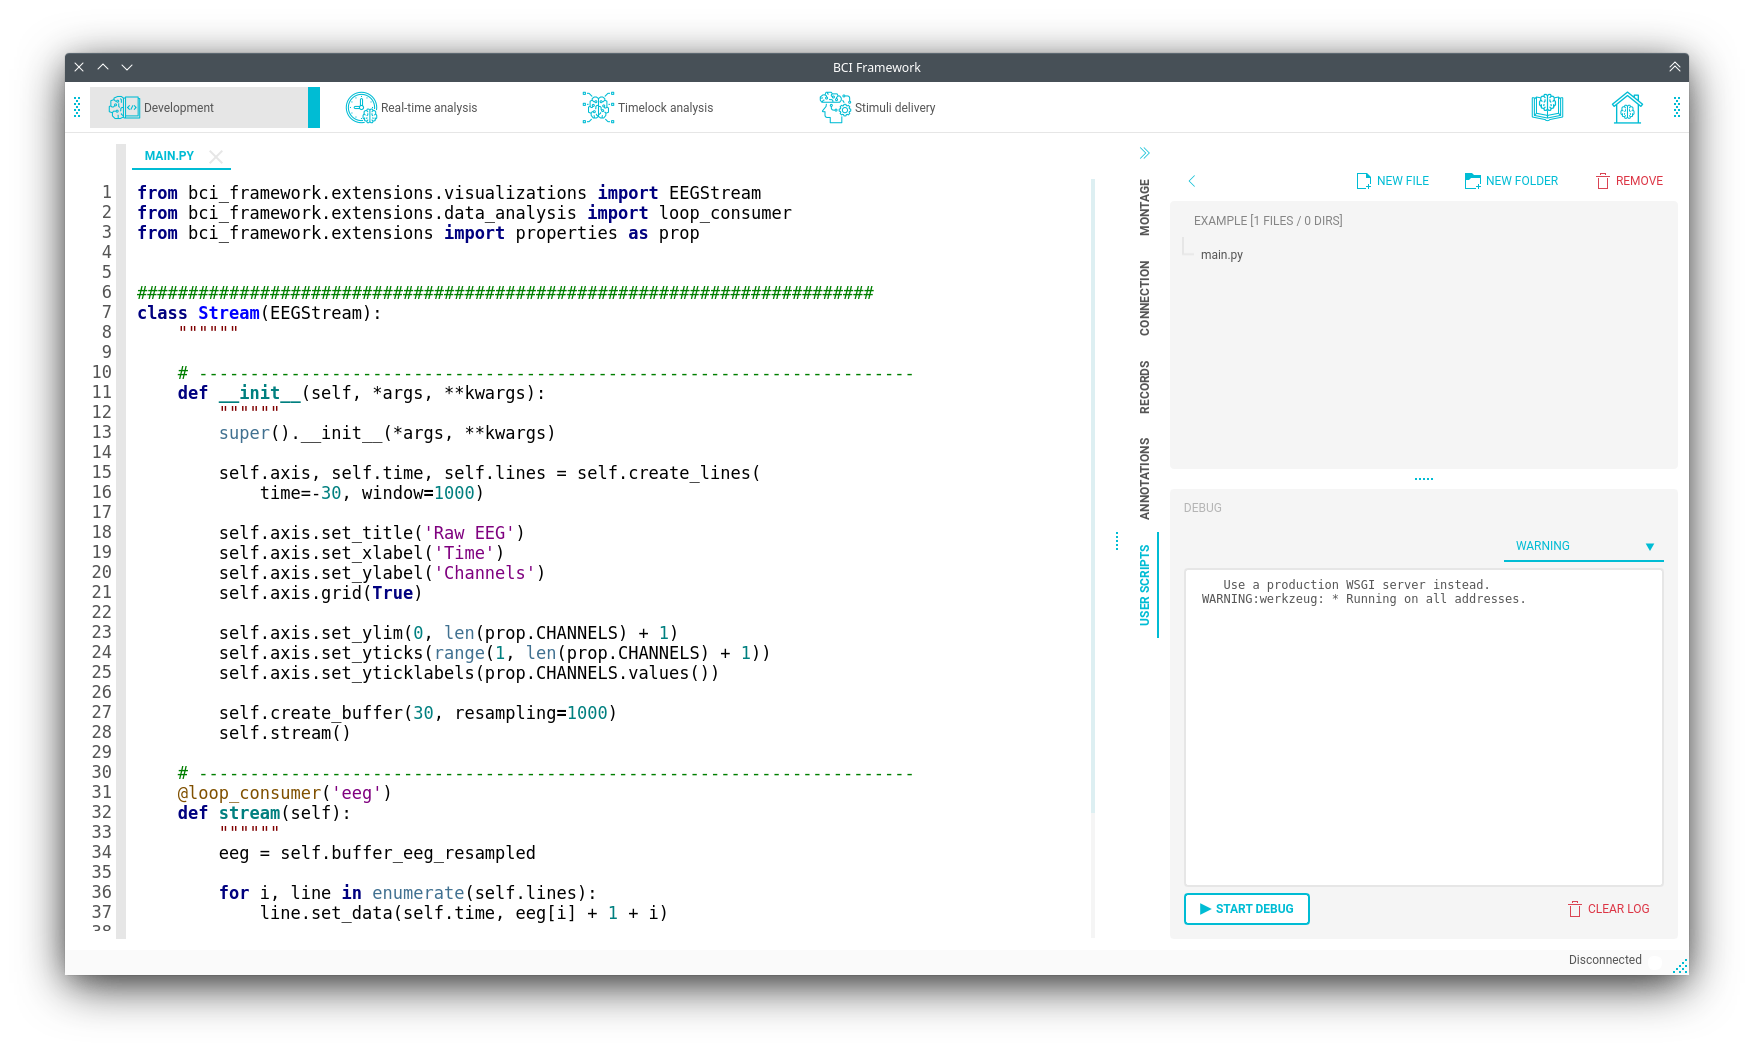
\includegraphics[width=0.8\textwidth]{Cap4/Figures/development_environment.png}
\par\end{centering}
\caption[BCI-Framework: integrated development environment]{BCI-Framework: Integrated development environment with previsualization area and debug console.}
\label{fig:development_environment}
\end{figure}



%======================================================================
\section{Real-time data analysis} \label{ch4:rt_data_analysis}  %(i.1)

The data analysis is powered by all \textit{Python} modules and the wrapped ones. This language has showed, to be a good choice for research and develop neuroscience implementations \cite{muller2015python}. Currently there are a bunch of modules like \footcite{MNE}{https://mne.tools/} specifically designed for exploring, visualizing, and analyzing human neurophysiological data. Alongside, much other that can be used to implement custom analysis like \footcite{Numpy}{https://numpy.org/} and \footcite{Scipy}{https://scipy.org/}, or for implement machine learning approaches like \footcite{Scikit-learn}{https://scikit-learn.org/} and \footcite{TensorFlow}{https://www.tensorflow.org/}.

% \textit{BCI-Framework} was designed in such a way that the user/researcher uses all this environment in combination with \gls*{EEG} signals and markers served at precise times without worry about the acquisition, synchronization and distribution. The real-time analysis is basically a \hyperref[]{Kafka consumer} or a \hyperref[]{Kafka transformer}, this component just connect with the stream that contain the \gls*{EEG} (or other signal) and consume the data to generate reports, local commands or send back a new kind of data to the stream.

\textit{BCI-Framework} was designed in such a way that the user/researcher can use the environment in combination with an easy to access \gls*{EEG} signals and markers to build their BCI system without care about the acquisition, synchronization and distribution. This approach allows to implement the real-time analysis as a basic \hyperref[]{Kafka consumer} or a \hyperref[]{Kafka transformer} that connect with the stream that contain the \gls*{EEG} (or other signal) and consume the data to serve the user/research and then generate reports, execute local commands or send back a new kind of data to the stream.

\begin{figure}
\begin{centering}
\includesvg[width=0.8\textwidth]{Cap4/Figures/kafka_transformer.svg}
\par\end{centering}
\caption[Kafka transformer]{Kafka transformer that generates a new kind of data (for example FFT) and stream it alongside the existent streams.}
\label{fig:transformer}
\end{figure}

For example, we can suppose that we need the \gls*{FFT} of the \gls*{EEG} signals in real-time, then, we can use a single script that calculate the \gls*{FFT} and create a new topic with the new data and stream it through all consumers. This transformer is graphically represented in Figure \ref{fig:transformer}, this script must run as an isolated process, and could be executed on any terminal of the network, the new data stream is automatically integrated and is available for all terminals.


%----------------------------------------------------------------------
\subsection{Data analysis scripting}\label{ch4:data_analysis}


The scripting consist of configure through a custom API the environment needed to read EEG signal. A bare minimum script looks like:

\begin{python}
from bci_framework.extensions.data_analysis import DataAnalysis

class Analysis(DataAnalysis):
    def __init__(self, *args, **kwargs):
        super().__init__(*args, **kwargs)

if __name__ == '__main__':
    Analysis()
\end{python}

The \quot{DataAnalysis} class includes a lot of useful methods to handle and configure the acquisition and manipulation of the data stream.

The API includes a custom decorator called \quot{loop\_consumer}, that is used to access asynchronously to the data stream. on every \quot{'eeg'} and \quot{'marker'} incoming data, this strings represents \textit{Kafka} topics. The \quot{stream} method only needs to be called a single time, after that, the decorator takes control of the executions, this means that entire script must finish with the call of the decorated method, in the constructor method. Is not possible, to use the decorator \quot{loop\_consumer} in more than one place, so the argument \quot{topic} could be used to create a flow control.

\begin{minted}
[
mathescape=true, 
xleftmargin=1cm, 
xrightmargin=1cm,
fontsize=\scriptsize, 
baselinestretch=1.2,
python3=true,
%  samepage=true,
% linenos=true,
highlightlines={6-10},
style=emacs,
highlightcolor=UN_primary!20,
]
{python}
from bci_framework.extensions.data_analysis import DataAnalysis, loop_consumer

class Analysis(DataAnalysis):
    def __init__(self, *args, **kwargs):
        super().__init__(*args, **kwargs)
        self.stream()

    @loop_consumer('eeg', 'marker')
    def stream(self):
        print('Incoming data...')

if __name__ == '__main__':
    Analysis()
\end{minted}

The decorated method receives five optional arguments: \quot{data}, \quot{topic}, \quot{frame}, \quot{latency} and \quot{kafka\_stream}. This arguments are defined in the wrapped decorator definition that is the reason why there is no arguments in the initial caller. This arguments works like inputs, and are optional, if some one is not declared then that local variable will be not created.

\begin{python}
@loop_consumer('eeg', 'aux')
def stream(self, data, topic, frame, latency):
    print(f'Incoming data #{frame}')
    
    match topic:
        case 'eeg':
            print(f'EEG{data.shape}')
        case 'aux':
            print(f'AUX{data.shape}')
    
    print(f'Topic: {topic}')
    print(f'Latency: {latency}')
\end{python}

\begin{python}
@loop_consumer('eeg', 'aux', 'marker')
def stream(self, topic):
    match topic:
    
        case 'eeg':
            print("EEG data incomming...")
            
        case 'aux':
            print("AUX data incomming...")

        case 'marker':
            print("Marker incomming...")
\end{python}

This scripting define the methods to subscribe to the Kafka stream topics. This solve issue about the access to the real-time data stream, however a high-level methods are also available to process, crop and buffer data.

%----------------------------------------------------------------------
\subsubsection{Buffering}

For real-time analysis, additionally to subscribe and acquire data from topics, is required a method to handle the buffer of the data acquired. The \quot{create\_buffer} method is used to configure the retention of the data streamed.

\begin{python}
self.create_buffer(seconds=30, fill=0)
\end{python}

The previous command will create a buffer of 30 seconds filled with 0 by default, the size of the buffer depends of the sampling rate and the number of the channels, this information is obtained from the framework parameters. 

\begin{minted}
[
mathescape=true, 
xleftmargin=1cm, 
xrightmargin=1cm, 
fontsize=\scriptsize, 
baselinestretch=1.2,
python3=true,
%  samepage=true,
% linenos=true,
highlightlines={4, 11-12},
style=emacs,
highlightcolor=UN_primary!20,
]
{python}
class Analysis(DataAnalysis):
    def __init__(self, *args, **kwargs):
        super().__init__(*args, **kwargs)
        self.create_buffer(seconds=30, fill=0)
        self.stream()

    @loop_consumer('eeg', 'aux')
    def stream(self):
        
        #  Buffer: all data from the last 30 seconds
        eeg = self.buffer_eeg
        aux = self.buffer_aux
         
        print(f'EEG{eeg.shape}')
        print(f'AUX{aux.shape}')
\end{minted}

Notice that the previous script has not argument in the decorated method, and that the buffer is accessible through the \quot{self.buffer\_eeg} and \quot{self.buffer\_aux} instance attributes.


%----------------------------------------------------------------------
\subsubsection{Resampling}

A sample length fixed will be created with the argument \quot{resampling}, by default is 1000 samples. A buffer for the auxiliary data with the same features is also generated. The buffering process is transparent for the user, once defined with \quot{create\_buffer} this will be automatically updated.

\begin{minted}
[
mathescape=true, 
xleftmargin=1cm, 
xrightmargin=1cm, 
fontsize=\scriptsize, 
baselinestretch=1.2,
python3=true,
%  samepage=true,
% linenos=true,
highlightlines={4, 12-13},
style=emacs,
highlightcolor=UN_primary!20,
]
{python}
class Analysis(DataAnalysis):
    def __init__(self, *args, **kwargs):
        super().__init__(*args, **kwargs)
        self.create_buffer(seconds=30, fill=0, resampling=1000)
        self.stream()

    @loop_consumer('eeg', 'aux')
    def stream(self):
        
        # Resampled buffer: 
        # the data from the last 30 seconds in a vector of 1000 samples
        eeg_r = self.buffer_eeg_resampled
        aux_r = self.buffer_aux_resampled
         
        print(f'EEG{eeg_r.shape}')
        print(f'AUX{aux_r.shape}')
\end{minted}

The resampled timeseries use the \quot{self.buffer\_eeg\_resampled} and \quot{self.buffer\_aux\_resampled} instance attributes.


%----------------------------------------------------------------------
\subsubsection{Data slicing referenced by markers}

This feature works similar to \quot{loop\_consumer}, but instead of return the latest block of data, the \quot{marker\_slicing} method return a \textit{trial}. A \textit{trial} is localized by almost one marker, and a margin time previous and posterior to the marker. 

\begin{minted}
[
mathescape=true, 
xleftmargin=1cm, 
xrightmargin=1cm, 
fontsize=\scriptsize, 
baselinestretch=1.2,
python3=true,
%  samepage=true,
% linenos=true,
highlightlines={11-12},
style=emacs,
highlightcolor=UN_primary!20,
]
{python}
from bci_framework.extensions.data_analysis import DataAnalysis, marker_slicing

class Analysis(DataAnalysis):
    def __init__(self, *args, **kwargs):
        super().__init__(*args, **kwargs)

        # Needs to be greater than the duration of the slice.
        self.create_buffer(seconds=30, aux_shape=3)
        self.slicing()

    @marker_slicing(['Right', 'Left'], t0=-2, duration=6)
    def slicing(self, eeg, aux, timestamp, marker):

        print(eeg.shape)
        print(aux.shape)
        print(timestamp.shape)
        print(marker)
        print()

if __name__ == '__main__':
    Analysis()
\end{minted}

In the previous script we are capturing trials of 6 seconds duration around the markers \quot{'Right'} and \quot{'Left'}. This feature is useful for debugging purposes, and synchronous paradigms with explicit markers presence, like \gls*{ERP}.


%----------------------------------------------------------------------
\subsubsection{Feed the stream using Kafka producer}

The data analysis can also works as a \textit{Kafka} producer, this feature is used to generate \textit{commands}, \textit{annotations}, \textit{feedbacks} and any other type of data under custom topics.

\begin{minted}
[
mathescape=true, 
xleftmargin=1cm, 
xrightmargin=1cm,
fontsize=\scriptsize, 
baselinestretch=1.2,
python3=true,
%  samepage=true,
% linenos=true,
highlightlines={8},
style=emacs,
highlightcolor=UN_primary!20,
]
{python}
from bci_framework.extensions.data_analysis import DataAnalysis

class Analysis(DataAnalysis):
    def __init__(self, *args, **kwargs):
        super().__init__(*args, **kwargs)

if __name__ == '__main__':
    Analysis(enable_produser=True)
\end{minted}

Once activate the producer, the \quot{send\_command}, \quot{send\_feedback} and \quot{send\_annotation} methods are available.

\begin{python}
# Command
self.send_command('MyCommand', value=45)

# Annotation
self.send_annotation('The subject yawn', duration=5)

# Feedback
feed = {'var1': 0,
        'var2': True,
        'var3': 'Right',
       }
self.send_feedback(**feed)

# send_feedback method are keyword arguments only
self.send_feedback(a=0, b=2.3, c='Left')

# Custom topic
self.generic_produser('my_topic', my_data)

\end{python}

The \quot{generic\_produser} method can be used to stream any custom data under a user defined topic. 
% The difference with the methods to stream \textit{commands}, \textit{annotations}, and \textit{feedbacks} resides on that the framework will interprets this lasts using specific process, and sometimes could execute instruction over the framework itself.

% %----------------------------------------------------------------------
% \subsection{Default data analysis}


%======================================================================
\section{Real-time visualization}  %(i.2)

The visualizations works very similar that the \hyperref[ch4:rt_data_analysis]{Real-time analysis}, with the difference that only comprise \hyperref[]{Kafka consumers} due the visualization is indented to be displayed inside of the \textit{BCI-Framework} interface and over a \textit{HTTP} protocol instead to create a new kind of data stream. 

\begin{figure}
\begin{centering}
\includesvg[width=0.8\textwidth]{Cap4/Figures/kafka_consumer.svg}
\par\end{centering}
\caption[kafka consumer]{Kafka consumer that access to the real-time EEG stream and use the data to perform individual process.}
\label{fig:transformer}
\end{figure}

The real-time visualizations consists of a computational process that manipulate the data in order to create static visualization and then update this one consecutively. The environment to create visualizations automatically serve the real-time EEG stream, then the user only must comply about the visualizations.


%----------------------------------------------------------------------
\subsection{Data visualization scripting}\label{ch4:viz_development}%(i.2)

Data visualization are based on \hyperref[appendix:matplotlib-figurestream]{Matplotlib-FigureStream}, this interface inherits all features from it and extends the utilities with an specific ones. Additionally all topics explained in \hyperref[ch4:data\_analysis]{Real-time analysis development} are valid here too, since visualizations is a special case of real-time analysis.

\begin{minted}
[
mathescape=true, 
xleftmargin=1cm, 
xrightmargin=1cm,
fontsize=\scriptsize, 
baselinestretch=1.2,
python3=true,
%  samepage=true,
% linenos=true,
highlightlines={4,17},
style=emacs,
highlightcolor=UN_primary!20,
]
{python}
from bci_framework.extensions.visualizations import EEGStream
from bci_framework.extensions.visualizations.utils import loop_consumer

class Stream(EEGStream):  # This is `matplotlib.Figure` based class
    def __init__(self):
        super().__init__()

        self.axis = self.add_subplot(111)
        self.axis.set_title('Title')
        self.axis.set_xlabel('Time')
        self.axis.set_ylabel('Amplitude')
        self.axis.grid(True)
        self.stream()

    @loop_consumer('eeg')
    def stream(self, *args, **kwargs):
        self.feed()

if __name__ == '__main__':
    Stream()
\end{minted}

Here the main difference is the class to heritage, \quot{EEGStream}, and the \quot{self.feed()} method. In this bare minimum example the constructor generates an empty plot using standard \textit{matplotlib} and them the \quot{loop\_consumer} will serve the data to the developer disposition.
% There is no limitations about the kind of plot that can be implemented here, only the ones related with performance.

\begin{python}
@loop_consumer('eeg')
def stream(self, data):
    eeg, aux = data

    ch0 = eeg[0]  # first eeg channel
    self.line.set_ydata(ch0)
    self.axis.set_ylim(ch0.min(), ch0.max())

    time = range(len(ch0))  # time axis
    self.line.set_xdata(time)
    self.axis.set_xlim(time[0], time[-1])

    self.feed()
\end{python}

The \quot{loop\_consumer} is used to update asynchronously the plot, since this method is executed on every new package received, this continuous update will create a plotting animation. The \quot{self.feed()} method send an update to the plotting stream server.

% %----------------------------------------------------------------------
% \subsection{Default data visualization}


%======================================================================
\section{Stimuli delivery} %(iii)

The interface for stimuli delivery is the only that interact directly with the \textit{patient}, neurophysiological experiments requires a controlled environment with the purpose to decrease the artifacts \cite{vialatte2008eeg, gomez2006automatic} in the signal as well as keep the patient concentrated on his task. This requirements suggest that the stimuli delivery must work over a remote presentation system and, in this way, separate physically the \textit{user} from the \textit{patient}. The method selected to develop an environment with these features was the classic web application based on HTML, CSS and JavasScript through the implementation of the \hyperref[appendix:brython-radiant]{Brython-Radiant framework}.

Although this is a common feature in almost all neurophysiological experiments designer software, after a series of observations and experience acquiring databases for the SPGR, we propose a brand new environment for the design, implementation and configuration of audio-visual stimuli delivery. Our interface able to the user to design flexible experiments and change the parameter easy and quickly without reprogramming the paradigm. Also, since the acquisition interface is integrated into the framework the database is generated automatically with all respective metadata and synchronized markers. Then the user only has to worry about the experiment while the database is generated in second plane.

\begin{figure}
\begin{centering}
% \includesvg[width=0.8\textwidth]{Cap4/Figures/transformer.svg}
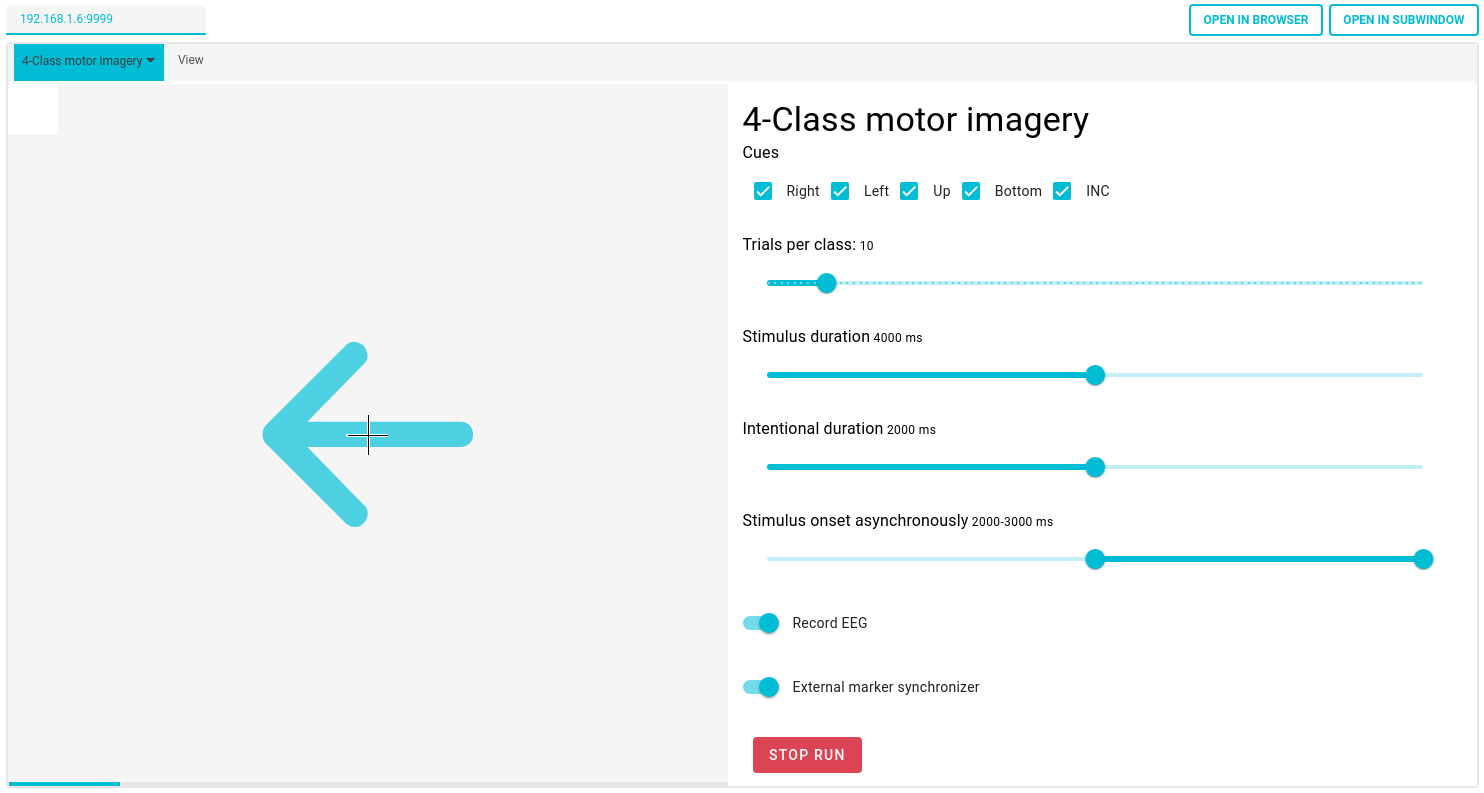
\includegraphics[width=0.8\textwidth]{Cap4/Figures/stimuli_delivery.png}
\par\end{centering}
\caption[Stimuli delivery interface]{Stimuli delivery interface, in the left the live view of the stimulus presented remotely to the patient, in the right the dashboard with the main parameter of the experiment.}
\label{fig:stimuli_delivery_interface}
\end{figure}

The proposal interface still requires that both, the stimuli delivery and the previsualization in the dashboard, update the screen synchronously. Then there are two kind of views, the first one is for the \textit{patient}, this view only includes the stimuli presentation and is the responsible to create the time markers. The second view is for the \textit{user}, additional to the stimuli preview also include a dashboard, this interface able to configure the experiment execution. 

%----------------------------------------------------------------------
\subsection{Stimuli delivery scripting}\label{ch4:stimuli_delivery_designer}%(iii)

This interface environment use \textit{Brython} and the \textit{Radiant framework} as backend for do the web development in a \textit{Python} style.

\begin{minted}
[
mathescape=true, 
xleftmargin=1cm, 
xrightmargin=1cm,
fontsize=\scriptsize, 
baselinestretch=1.2,
python3=true,
%  samepage=true,
% linenos=true,
highlightlines={3-5,12-17},
style=emacs,
highlightcolor=UN_primary!20,
]
{python}
from bci_framework.extensions.stimuli_delivery import StimuliAPI

# Brython modules
from browser import document, html
from browser.widgets.dialog import InfoDialog

class StimuliDelivery(StimuliAPI):
    def __init__(self, *args, **kwargs):
        super().__init__(*args, **kwargs)
        document.clear()

        # main brython code
        document.select_one('body') <= html.H3('Hello world')

        button = html.BUTTON('click me')
        button.bind('click', lambda evt: InfoDialog('Hello', 'world'))
        document.select_one('body') <= button

if __name__ == '__main__':
    StimuliDelivery()
\end{minted}

The \quot{StimuliAPI} includes lot of methods to simplify the interaction with the stimuli delivery environment


%----------------------------------------------------------------------
\subsubsection{Stimuli area and Dashboard}

One of the main features is the possibility to make configurable experiments, in favor to this philosophy, by default they are build both areas, \quot{self.stimuli\_area} and \quot{self.dashboard} in the class constructor.

% \begin{python}
self.stimuli_area <= html.H3('Stimuli area')
self.dashboard <= html.H3('Dashboard')

# Insert a cross in the middle of the stimuli area
self.show_cross()

# This area is used for external event processord
self.show_synchronizer()
\end{python}
% \begin{figure}
\begin{centering}
% \includesvg[width=0.8\textwidth]{Cap4/Figures/transformer.svg}
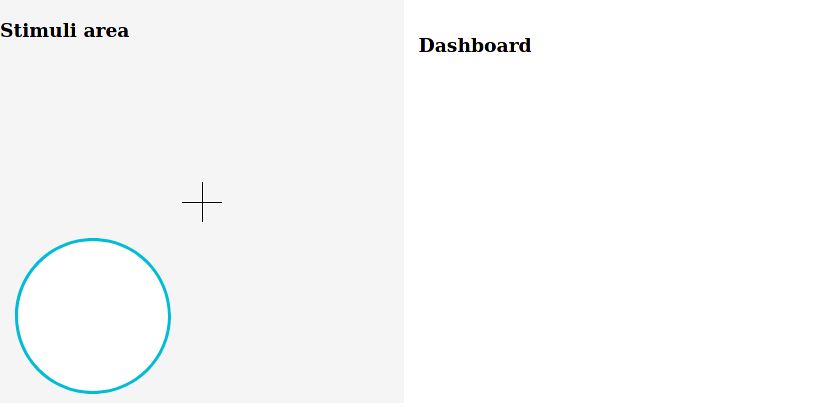
\includegraphics[width=0.8\textwidth]{Cap4/Figures/stimuli_delivery_areas.png}
\par\end{centering}
\caption[]{.}
\label{fig:stimuli_delivery_interface}
\end{figure}

The attempt use of the stimuli area is to use it to present the stimulus, this area is automatically duplicated in the remote patient view. The right side is intended to the dashboard, this layout is only accessible for the user, and is used to configure the experiment.

The both areas are accessible thought the class attribute \quot{self.stimuli\_area} and \quot{self.dashboard}, as instances of \quot{browser.html.DIV}. There is a particularity in the language about the use of \quot{<=} to nest elements.


%----------------------------------------------------------------------
\subsection{Widgets}

All widgets and styles are part of \footcite{Material Components Web}{https://material.io/develop/web} and can be implemented with a custom module implementation designed to display widgets and get values. All widgets are available troughs the \quot{Widgets} submodule located in the module \quot{bci\_framework.extensions.stimuli\_delivery.utils}.

\begin{python}
from bci_framework.extensions.stimuli_delivery.utils import Widgets as w
\end{python}

%----------------------------------------------------------------------
\subsubsection{Typography}
Not only for aesthetics, a default font was selected to make the messages easy to read, even on small screens, in combination with a set of hierarchies and contexts.
\begin{python}
self.dashboard <= w.label('headline1', typo='headline1')
self.dashboard <= w.label('headline2', typo='headline2')
self.dashboard <= w.label('headline3', typo='headline3')
self.dashboard <= w.label('headline4', typo='headline4')
self.dashboard <= w.label('headline5', typo='headline5')
self.dashboard <= w.label('headline6', typo='headline6')
self.dashboard <= w.label('body1', typo='body1')
self.dashboard <= w.label('body2', typo='body2')
self.dashboard <= w.label('subtitle1', typo='subtitle1')
self.dashboard <= w.label('subtitle2', typo='subtitle2')
self.dashboard <= w.label('caption', typo='caption')
self.dashboard <= w.label('button', typo='button')
self.dashboard <= w.label('overline', typo='overline')
\end{python}

\begin{figure}[H]
\begin{centering}
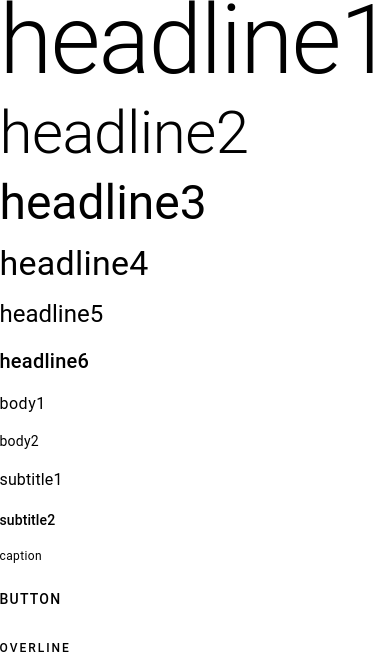
\includegraphics[scale=0.5]{Cap4/Figures/widgets/typography.png}
\par\end{centering}
\caption[Brython Radiant: Typography]{Brython Radiant: Default typography.}
\label{fig:radiant_typography}
\end{figure}

%----------------------------------------------------------------------
\subsubsection{Buttons}
The buttons have the action \quot{on\_click} associated, this action just trigger a method, a function or an anonymous function.
\begin{python}
    self.dashboard <= w.label('Buttons', typo='headline4', style=flex_title)
    self.dashboard <= w.button(
        'Button 1',
        style=flex,
        on_click=lambda: setattr(
            document.select_one('#for_button'), 'html', 'Button 1 pressed!'
        ),
    )
    self.dashboard <= w.button(
        'Button 2', style=flex, on_click=self.on_button2
    )
    self.dashboard <= w.label(
        f'', id='for_button', typo=f'body1', style=flex
    )

def on_button2(self):
    document.select_one('#for_button').html = 'Button 2 pressed!'
\end{python}


\begin{figure}[H]
\begin{centering}
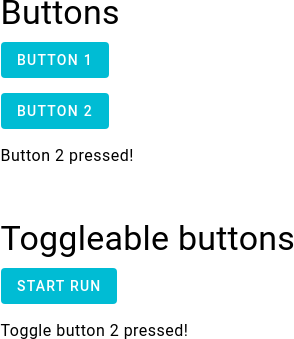
\includegraphics[scale=0.5, left]{Cap4/Figures/widgets/buttons.png}
\par\end{centering}
\caption[Brython Radiant: Buttons]{Brython Radiant: Buttons.}
\label{fig:radiant_buttons}
\end{figure}

%----------------------------------------------------------------------
\subsubsection{Switch}
The switch, like the button, have an action associated, but also, a state. The state can be getted on any moment using the \quot{id} with the method \quot{get\_value(id)} or in the argument of the binded action.
\begin{python}
    self.dashboard <= w.label('Switch', typo='headline4', style=flex_title)
    self.dashboard <= w.switch(
        'Switch 1', checked=True, on_change=self.on_switch, id='my_swicth'
    )
    self.dashboard <= w.label(
        f'', id='for_switch', typo=f'body1', style=flex
    )


def on_switch(self, value):
    # value = self.widgets.get_value('my_swicth')
    document.select_one('#for_switch').html = f'Switch Changed: {value}'
\end{python}


\begin{figure}[H]
\begin{centering}
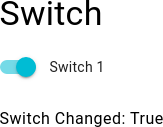
\includegraphics[scale=0.5]{Cap4/Figures/widgets/switch.png}
\par\end{centering}
\caption[Brython Radiant: Switch]{Brython Radiant: Switch.}
\label{fig:radiant_switch}
\end{figure}

%----------------------------------------------------------------------
\subsubsection{Checkbox}
Multiple selection list items use the checkbox to interact with this list of items, the state comprise the list of selected options, and \quot{on\_change} is triggered on every item status changed.
\begin{python}
    self.dashboard <= w.label('Checkbox', typo='headline4', style=flex_title)
    self.dashboard <= w.checkbox(
        'Checkbox',
        options=[[f'chb-{i}', False] for i in range(4)],
        on_change=self.on_checkbox,
        id='my_checkbox',
    )
    self.dashboard <= w.label(
        f'', id='for_checkbox', typo=f'body1', style=flex
    )


def on_checkbox(self):
    value = w.get_value('my_checkbox')
    document.select_one('#for_checkbox').html = f'Checkbox Changed: {value}'
\end{python}


\begin{figure}[H]
\begin{centering}
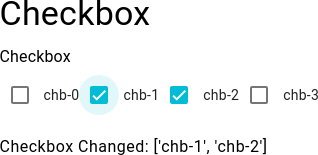
\includegraphics[scale=0.5]{Cap4/Figures/widgets/checkbox.png}
\par\end{centering}
\caption[Brython Radiant: Checkbox]{Brython Radiant: Checkbox.}
\label{fig:radiant_checkbox}
\end{figure}


%----------------------------------------------------------------------
\subsubsection{Radios}
Similar to checkboxes but, the selection is exclusive to only one item, then the state is a string.
\begin{python}
    self.dashboard <= w.label('Radios', typo='headline4', style=flex_title)
    self.dashboard <= w.radios(
        'Radios',
        options=[[f'chb-{i}', f'chb-{i}'] for i in range(4)],
        on_change=self.on_radios,
        id='my_radios',
    )
    self.dashboard <= w.label(
        f'', id='for_radios', typo=f'body1', style=flex
    )


def on_radios(self):
    value = w.get_value('my_radios')
    document.select_one('#for_radios').html = f'Radios Changed: {value}'
\end{python}


\begin{figure}[H]
\begin{centering}
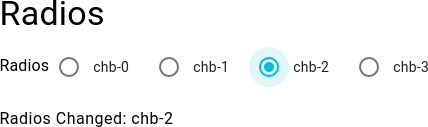
\includegraphics[scale=0.5]{Cap4/Figures/widgets/radios.png}
\par\end{centering}
\caption[Brython Radiant: Radios]{Brython Radiant: Radios.}
\label{fig:radiant_radios}
\end{figure}

%----------------------------------------------------------------------
\subsubsection{Select}
The select component comply the same function that the radios, but the interface is displayed to the user using a different widget. 
\begin{python}
    self.dashboard <= w.label('Select', typo='headline4', style=flex)
    self.dashboard <= w.select(
        'Select',
        [[f'sel-{i}', f'sel-{i}'] for i in range(4)],
        on_change=self.on_select,
        id='my_select',
    )
    self.dashboard <= w.label(
        f'', id='for_select', typo=f'body1', style=flex
    )


def on_select(self, value):
    # value = w.get_value('my_select')
    document.select_one('#for_select').html = f'Select Changed: {value}'
\end{python}


\begin{figure}[H]
\begin{centering}
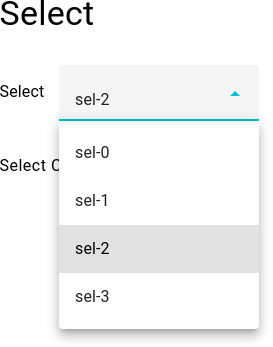
\includegraphics[scale=0.5]{Cap4/Figures/widgets/select.png}
\par\end{centering}
\caption[Brython Radiant: Select]{Brython Radiant: Select.}
\label{fig:radiant_select}
\end{figure}


%----------------------------------------------------------------------
\subsubsection{Sliders}
The slider are used to select numbers from a range or a range itself. The state is the value or the range and the trigger event is the continuous update, not the change after a release.
\begin{python}
    # Slider
    self.dashboard <= w.label('Slider', typo='headline4', style=flex)
    self.dashboard <= w.slider(
        'Slider',
        min=1,
        max=10,
        step=0.1,
        value=5,
        on_change=self.on_slider,
        id='my_slider',
    )
    self.dashboard <= w.label(
        f'', id='for_slider', typo=f'body1', style=flex
    )

    # Slider range
    self.dashboard <= w.label('Slider range', typo='headline4', style=flex)
    self.dashboard <= w.range_slider(
        'Slider range',
        min=0,
        max=20,
        value_lower=5,
        value_upper=15,
        step=1,
        on_change=self.on_slider_range,
        id='my_range',
    )
    self.dashboard <= w.label(f'', id='for_range', typo=f'body1', style=flex)


def on_slider(self, value):
    # value = w.get_value('my_slider')
    document.select_one('#for_slider').html = f'Slider Changed: {value}'


def on_slider_range(self, value):
    # value = w.get_value('my_slider')
    document.select_one('#for_range').html = f'Range Changed: {value}'
\end{python}


\begin{figure}[H]
\begin{centering}
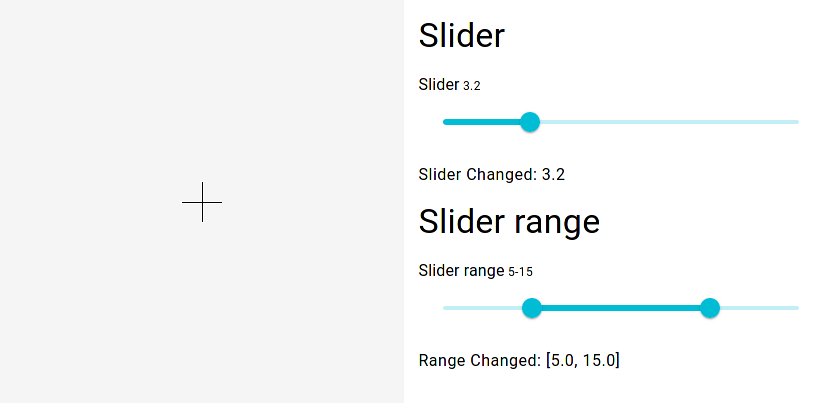
\includegraphics[scale=0.5]{Cap4/Figures/widgets/sliders.png}
\par\end{centering}
\caption[Brython Radiant: Slider]{Brython Radiant: Sliders.}
\label{fig:radiant_sliders}
\end{figure}

%----------------------------------------------------------------------
\subsection{Audiovisual stimuli}

Since Brython-Radiant is basically a frontend framework, all visual stimuli can be implemented through JavaScript, HTML, and CSS. Web applications are the most featured environ to develop audivisual stimuli. Present and update views, reproduce audio or video are basic tasks in this environment. 

%----------------------------------------------------------------------
\subsubsection{Tones and audio}

The \textit{Tone} library allows playing single notes using the \quot{javascript} \quot{AudioContext backend}, the duration and the gain can also be configured.
\begin{python}
from bci_framework.extensions.stimuli_delivery.utils import Tone as t

duration = 100
gain = 0.5

self.dashboard <= w.button(
    'f#4',
    on_click=lambda: t('f#4', duration, gain),
    style={'margin': '0 15px'},
)
self.dashboard <= w.button(
    'D#0',
    on_click=lambda: t('D#0', duration, gain),
    style={'margin': '0 15px'},
)
self.dashboard <= w.button(
    'B2',
    on_click=lambda: t('B2', duration, gain),
    style={'margin': '0 15px'},
)
\end{python}

The Audio module allows to reproduce complete audio files.
\begin{python}
from bci_framework.extensions.stimuli_delivery.utils import Audio as a

a.load('rain.wav')

self.dashboard <= w.label(
    'Audio',
    'headline4',
    style={
        'margin-bottom': '15px',
        'display': 'flex',
    },
)
self.dashboard <= html.BR()

self.dashboard <= w.slider(
    'Gain',
    min=0,
    max=1,
    step=0.1,
    value=0.5,
    id='gain',
    on_change=a.set_gain,
)

self.dashboard <= w.button(
    'Start', on_click=a.play, style={'margin': '0 15px'}
)
self.dashboard <= w.button(
    'Stop', on_click=a.stop, style={'margin': '0 15px'}
)

\end{python}

%----------------------------------------------------------------------
\subsubsection{Visual stimuli}

A complete free HTML-based environment available to design and implement neurophysiological experiments.

\begin{python}
from bci_framework.extensions.stimuli_delivery.utils import icons

self.dashboard <= icons.fa('fa-arrow-right')   # FontAwesome
self.dashboard  <= icons.bi('bi-arrow-right')  # Bootstrap icon
self.dashboard  <= icons.mi('face', size=24)   # Material icons 
\end{python}

%----------------------------------------------------------------------
\subsection{Stimuli delivery pipeline}

Pipelines consist of the controlled execution of methods with asynchronous timeouts. We define a paradigm as a sequence of trials, and each trial is composed of a sequence of parameterized views. 

For example, in the classic motor imagery paradigm with two classes, right and left. A trial is the presentation of one stimulus, each trial is composed of a sequence of views: clear screen, wait, show stimulus, clear screen. And then, the next trial with the same sequence of views but with different parameters, like the stimulus itself, or random waits.

This task can be implemented programmatically with the pipeline design pattern and simplified the implementation. First one we need to define the trials like a list of  parameter used for each one of the single trial. For example, here we define 3 trials:

\begin{python}
trials = [
    {'s1': 'Left',  # Trial 1
     'r1': 91,
     },

    {'s1': 'Right',  # Trial 2
     'r1': 85,
     },

    {'s1': 'Left',  # Trial 3
     'r1': 30,
     },
]
\end{python}

And the trial views consists of a list of sequential methods with a respective timeout (method, timeout), if the timeout is a number then this will indicate the milliseconds until the next method call. If the timeout is a list, then a random (with uniform distribution) number between that range will be generated on each trial.

\begin{python}
view = [
    (self.view1, 500),
    (self.view2, [500, 1500]),
    (self.view3, w.get_value('slider')),
    (self.view4, w.get_value('range')),
]
\end{python}

The view configuration can used states from widgets by referencing the \quot{id} instead of an explicit value:

\begin{python}
view = [
    (self.view1, 500),          # timeout
    (self.view2, [500, 1500]),  # range
    (self.view3, 'slider'),     # from widgets id
    (self.view4, 'range'),
]
\end{python}

Then, we need to define the views methods, each method  is a step needed to build a single trial. By definition, all views will share the same arguments, even if they are not used by that method.
 
\begin{python}
def view1(self, s1, r1):
    print(f'On view1: {s1=}, {r1=}')

def view2(self, s1, r1):
    print(f'On view2: {s1=}, {r1=}')

def view3(self, s1, r1):
    print(f'On view3: {s1=}, {r1=}')

def view4(self, s1, r1):
    print(f'On view4: {s1=}, {r1=}\n')
\end{python}

Finally, our pipeline can be executed with the method \quot{self.run\_pipeline}:

\begin{python}
self.run_pipeline(view, trials)
\end{python}

Here, the pipeline is running all tree trials and for each one the four views, notice that each view receive all the parameter that configure the single trial. 

\begin{python}
On view1: s1=Left, r1=91
On view2: s1=Left, r1=91
On view3: s1=Left, r1=91
On view4: s1=Left, r1=91

On view1: s1=Right, r1=85
On view2: s1=Right, r1=85
On view3: s1=Right, r1=85
On view4: s1=Right, r1=85

On view1: s1=Left, r1=30
On view2: s1=Left, r1=30
On view3: s1=Left, r1=30
On view4: s1=Left, r1=30
\end{python}

In addition to handle the organization and planning execution of the trials, the main purpose of the pipelines is to synchronize the remote presentation. Figure \ref{fig:pipelines} shows the composition of a basic trial, each view needs a time to complete their execution, the pipeline system ensure that times the between $T0-T1$, $T1-T2$, and $T2-T3$, remains the same for all executions, no matter the fluctuations of the view execution.

\begin{figure}
\begin{centering}
\includesvg[width=1\textwidth]{Cap4/Figures/pipelines.svg}
\par\end{centering}
\caption[Stimuli delivery pipeline]{Each trial is composed of views, the pipelines features define the asynchronous execution of each view at the precise time.}
\label{fig:pipelines}
\end{figure}





%----------------------------------------------------------------------
\subsection{Hardware-based event synchronization}

The stimuli delivery interface integrate a physical method to synchronize markers, this method used an small portion of the same screen that present the stimulus. In this area a sensor is attached and connected directly with the acquisition system in order to obtain a single stream with both signals, EEG and the external ones using the \textit{analog boardmode} supported by \textit{OpenBCI}.

% %----------------------------------------------------------------------
% \subsection{Default stimuli delivery paradigms}


%======================================================================
\section{Markers, commands, annotations and feedbacks}

In order to integrate and intercommunicate all environments a set of custom channels for messaging was defined, this commands are functional in all environs: Data analysis, visualization and Stimuli delivery. The \textit{markers}, \textit{annotations}, and \textit{feedbacks} interacts internally in the framework in order to configure the framework, intercommunicate process or create registers over the acquired signal. Unlike \textit{commands} that consist of a simple recommendation to standardize the interaction of the framework environment with external process.

%----------------------------------------------------------------------
\subsubsection{Markers}

Used to define events over the EEG signal, needs a label and optionally a blink time in milliseconds.
\begin{python}
self.send_marker("MARKER")
self.send_marker("MARKER", blink=200)
\end{python}
The timestamp for each marker is generated internally in order to the use the main Kafka clock reference, this strategy avoids to use multiple clocks sources and generate latencies with differents trends. Large latency with small jitter is always preferred over small latency with large jitter.


%----------------------------------------------------------------------
\subsubsection{Annotations}

Used to define events over the patient, needs a description and optionally a duration.
\begin{python}
self.send_annotation('Data record start')
self.send_annotation('The subject yawn', duration=5)
\end{python}
This format is exported to the EDF standard annotations. Like in markers the timestamp is generated internally.


%----------------------------------------------------------------------
\subsubsection{Commands}

This is a private framework topic defined in Kafka used to share information with external devices, the main purpose is about to close the loop for complete BCI systems. Need a label and a value, the value can be also any Python data structure.
\begin{python}
self.send_command('MyCommand', value=45)
self.send_command('MyCommand', value={'A':45, 'B':12})
\end{python}
This messages use the \quot{'command'} topic to share the information. 

%----------------------------------------------------------------------
\subsubsection{Feedbacks}\label{ch4:feedbacks}

The feedbacks are used to communicate the Data analysis and Data visualizations with the Stimuli Delivery platform with asynchronous callbacks. For this purpose, there is a predefined stream channel called feedback. This is useful to develop Neurofeedback applications.

The asynchronous handler can be configured with the Feedback class:
\begin{python}
from bci_framework.extensions.stimuli_delivery import Feedback
\end{python}

This object needs an identifier and optionally callback method to handle the input messages.
\begin{python}
self.feedback = Feedback(self, 'my_feedback_id')  # ID
self.feedback.on_feedback(self.on_input_feedback)  #callback
\end{python}

The callback method will receive the input data as keyword only arguments.
\begin{python}
def on_input_feedback(self, **feedback):
    ...
\end{python}

And the method \quot{self.feedback.write} is the intented way to send feedbacks to the complementary environment.
\begin{python}
self.feedback.write(**feedback)
\end{python}

This code structure must be on both endpoints, with the same \textit{ID} in order to communicate them and exchange feedback information

%======================================================================
\section{Latency analysis and event marker synchronization}

% Here the \textit{offset} is the difference between the timestamp of the marker (send by software) asosiated with a stimulus and the real moment when the stimulus is showed to the \textit{patient}. Is possible to take advantage of the \textit{OpenBCI} construction, this board includes a set of analog and digital inputs that can be used to synchronize this events. We only need an \gls*{LDR} module connected to the pin \textit{D11} (or \textit{A5}) and the board must be configured on  \textit{analog mode}.

Is possible to take advantage of the OpenBCI implementation, this board includes a set of analog and digital inputs that can be used to synchronize markers. In order to use OpenBCI, we will only need an \gls*{LDR} module connected to the pin D11 (or A5) and start the automatic latency correction system included in BCI-Framework. 

\begin{figure}
\begin{centering}
% \includesvg[width=0.8\textwidth]{Cap4/Figures/transformer.svg}
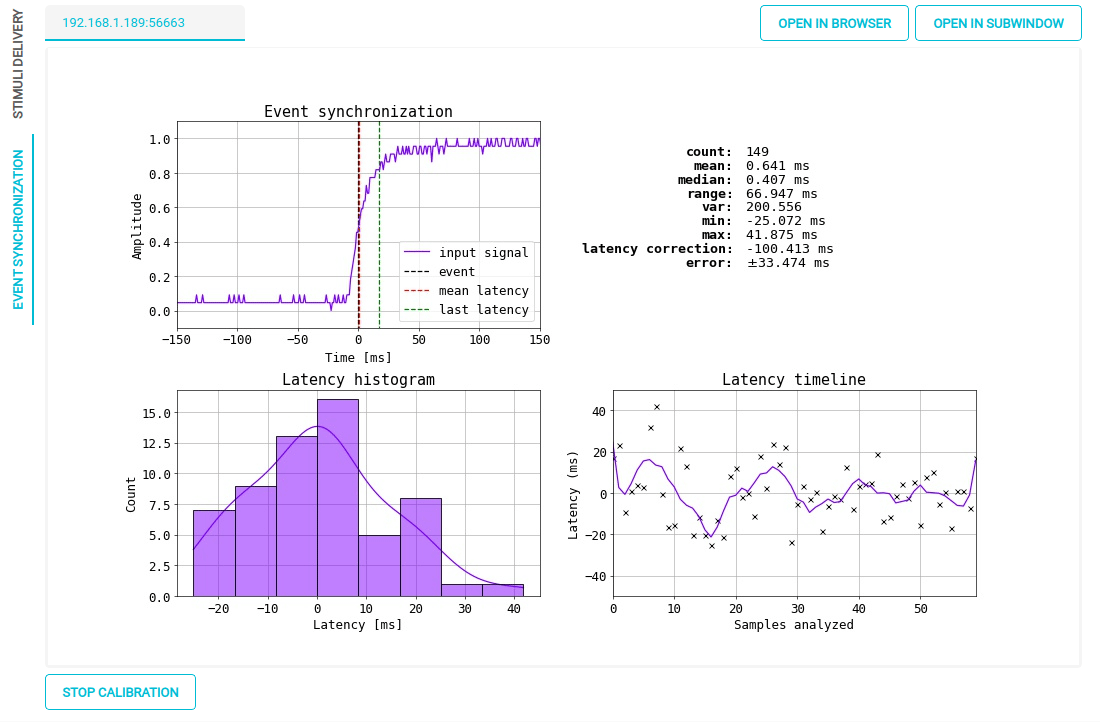
\includegraphics[width=0.8\textwidth]{Cap4/Figures/marker_sync.png}
\par\end{centering}
\caption[BCI-Framework: Marker synchronization]{BCI-Framework: Marker synchronization real-time interface.}
\label{fig:marker_sync}
\end{figure}

BCI-Framework integrates an interface to measure latencies and synchronize markers (Figure \ref{fig:marker_sync}), it was designed to be used on distributed environments. This simple latency correction consists of a stimuli delivery with only a marker synchronization area, the \gls*{LDR} module is constantly sensing (the boardmode must be in analog mode) so the changes on the square signal are compared with streamed markers and then the latency is corrected. The latency correction only affects the current instance, if BCI-Framework is restarted this calibration will be lose. For hard event synchronization, is prefer to use the markers synchronization constantly during all session.


%======================================================================
\section{Close the loop and Neurofeedback}

The BCI application with a close loop implementation consist of process in real-time the acquired data in order to execute commands in the real world. Although physiologically the close-loop signals differs from neurofeedback signals, since the nature of the data is different, the programmatically handle is exactly the same and are handled by \hyperref[ch4:feedbacks]{Feedbacks}. Once the feedback is defined through a method to perform asynchronous communication between them, the neurofeedback approaches can be implemented using this features. This implementation can be designed to run inside the interface, using \hyperref[ch4:rt_data_analysis]{Real-time data analysis} or to run isolated in no contextualized process. In Appendix \ref{appendix:neurofeedback} shows the implementation of a neurofeedback system.

The advantage to run process inside the framework is that this scrips share all the environment variables, and can be monitored through the main interface. On the other hand the scripts that run outside the framework only have access to the Kafka streams, this means that only can use the acquire data and are agnostics about everything else.




%======================================================================
\section{Summary and discussion}

BCI-Framework is the convergence of a set of drivers and tools working together to serve to the \textit{user} a full environment to acquire EEG signals and perform neurophysiological experiments with reliability and flexibility. Advance user can use the framework to develop custom visualizations and design paradigms that satisfy their needs using the integrated development environment. The main development was performed using Python, this feature brings to the framework one of the most complete computational libraries to work with data analysis and machine learning highly used to develop \gls*{BCI} systems today. 

The integrated development environment serve a full \gls*{API} with the main tasks automatized. The real-time data analysis and visualization build in background a fast system to buffering, sub-sampling and slice incoming EEG data en real-time. The stimuli delivery scripting has been designed to present views to the \textit{patient} asynchronously. In all cases the \textit{developer} only must care about the specific implementation of the analysis, visualizations and paradigm designed.

However the system only supports one acquisition board, \textit{OpenBCI Cyton}, although this is one of the most flexible and featured options available at the moment to write this thesis, the spreading of the framework tool could be seriously compromised. Also the main operating system focused, any based on \textit{GNU/Linux}, could be a reason that limits the adoption of the framework by the community.

